\documentclass{vkr}
\usepackage[english, russian]{babel} % переносы
\usepackage{graphicx} % для вставки картинок
\graphicspath{{images/}} % путь к изображениям
\usepackage[hidelinks]{hyperref}
\usepackage{float} % определяет метод H для рисунка с переносом на следующую страницу, ели не помещается
\usepackage{pdflscape}
\addto{\captionsrussian}{\renewcommand{\refname}{СПИСОК ИСПОЛЬЗОВАННЫХ ИСТОЧНИКОВ}}
\usepackage{xltabular} % для вставки таблиц
\usepackage{makecell}
\renewcommand\theadfont{} % шрифт в /thead
\usepackage{array} % для определения новых типов столбцов таблиц
\newcolumntype{T}{>{\centering\arraybackslash}X} % новый тип столбца T - автоматическая ширина столбца с выравниванием по центру
\newcolumntype{R}{>{\raggedleft\arraybackslash}X} % новый тип столбца R - автоматическая ширина столбца с выравниванием по правому краю
\newcolumntype{C}[1]{>{\centering\let\newline\\\arraybackslash\hspace{0pt}}m{#1}} % новый тип столбца C - фиксированная ширина столбца с выравниванием по центру
\newcolumntype{r}[1]{>{\raggedleft\arraybackslash}p{#1}} % новый тип столбца r - фиксированная ширина столбца с выравниванием по правому краю
\newcommand{\centrow}{\centering\arraybackslash} % командой \centrow можно центрировать одну ячейку (заголовок) в столбце типа X или p, оставив в оcтальных ячейках другой тип выравнивания
\newcommand{\finishhead}{\endhead\hline\endlastfoot}
\newcommand{\continuecaption}[1]{\caption*{#1}\\ \hline }
\usepackage{etoolbox}
\AtBeginEnvironment{xltabular}{\refstepcounter{tablecnt}} % подсчет таблиц xltabular, обычные таблицы подсчитываются в классе

\usepackage[tableposition=top]{caption} % подпись таблицы вверху
\captionsetup{strut=off}
\setlength{\intextsep}{0pt} % Vertical space above & below [h] floats
\setlength{\textfloatsep}{0pt} % Vertical space below (above) [t] ([b]) floats
\DeclareCaptionLabelFormat{gostfigure}{Рисунок #2} %подпись рисунка
\DeclareCaptionLabelFormat{gosttable}{Таблица #2} %подпись таблицы
\DeclareCaptionLabelSeparator{gost}{~--~} %разделитель в рисунках и таблицах
\captionsetup{labelsep=gost}
\captionsetup[figure]{aboveskip=10pt,belowskip=4mm,justification=centering,labelformat=gostfigure} % настройка подписи рисунка
\captionsetup[table]{font={stretch=1.41},skip=0pt,belowskip=0pt,aboveskip=8.5pt,singlelinecheck=off,labelformat=gosttable} % настройка подписи таблицы

\setlength{\LTpre}{8mm} % отступ сверху таблицы
\setlength{\LTpost}{6mm} % отступ снизу таблицы

\usepackage{enumitem}
\setlist{nolistsep,wide=\parindent,itemindent=*} % отступы вокруг списков, выравнивание с учетом разделителя

\usepackage{color} %% это для отображения цвета в коде
\usepackage{listings} %% листинги кода
\setmonofont[Scale=0.7]{Verdana} % моноширный шрифт для листинга

\definecolor{codegreen}{rgb}{0,0.6,0}
\definecolor{codegray}{rgb}{0.5,0.5,0.5}
\definecolor{codepurple}{rgb}{0.58,0,0.82}

\lstset{ %
language=C,                 % выбор языка для подсветки (здесь это С)
numbers=left,               % где поставить нумерацию строк (слева\справа)
numberstyle=\tiny,           % размер шрифта для номеров строк
stepnumber=1,                   % размер шага между двумя номерами строк
numbersep=5pt,                % как далеко отстоят номера строк от подсвечиваемого кода
commentstyle=\color{codegreen},
keywordstyle=\color{magenta},
numberstyle=\tiny\color{codegray},
stringstyle=\color{codepurple},
basicstyle=\linespread{0.95}\ttfamily,
backgroundcolor=\color{white}, % цвет фона подсветки - используем \usepackage{color}
showspaces=false,            % показывать или нет пробелы специальными отступами
showstringspaces=false,      % показывать или нет пробелы в строках
showtabs=false,             % показывать или нет табуляцию в строках
frame=single,              % рисовать рамку вокруг кода
tabsize=2,                 % размер табуляции по умолчанию равен 2 пробелам
captionpos=t,              % позиция заголовка вверху [t] или внизу [b] 
breaklines=true,           % автоматически переносить строки (да\нет)
breakatwhitespace=false, % переносить строки только если есть пробел
escapeinside={\%*}{*)}   % если нужно добавить комментарии в коде
}

\makeatletter % чтобы допускались русские комментарии в листингах
\lst@InputCatcodes
\def\lst@DefEC{%
 \lst@CCECUse \lst@ProcessLetter
  ^^80^^81^^82^^83^^84^^85^^86^^87^^88^^89^^8a^^8b^^8c^^8d^^8e^^8f%
  ^^90^^91^^92^^93^^94^^95^^96^^97^^98^^99^^9a^^9b^^9c^^9d^^9e^^9f%
  ^^a0^^a1^^a2^^a3^^a4^^a5^^a6^^a7^^a8^^a9^^aa^^ab^^ac^^ad^^ae^^af%
  ^^b0^^b1^^b2^^b3^^b4^^b5^^b6^^b7^^b8^^b9^^ba^^bb^^bc^^bd^^be^^bf%
  ^^c0^^c1^^c2^^c3^^c4^^c5^^c6^^c7^^c8^^c9^^ca^^cb^^cc^^cd^^ce^^cf%
  ^^d0^^d1^^d2^^d3^^d4^^d5^^d6^^d7^^d8^^d9^^da^^db^^dc^^dd^^de^^df%
  ^^e0^^e1^^e2^^e3^^e4^^e5^^e6^^e7^^e8^^e9^^ea^^eb^^ec^^ed^^ee^^ef%
  ^^f0^^f1^^f2^^f3^^f4^^f5^^f6^^f7^^f8^^f9^^fa^^fb^^fc^^fd^^fe^^ff%
  ^^^^20ac^^^^0153^^^^0152%
  % Basic Cyrillic alphabet coverage
  ^^^^0410^^^^0411^^^^0412^^^^0413^^^^0414^^^^0415^^^^0416^^^^0417%
  ^^^^0418^^^^0419^^^^041a^^^^041b^^^^041c^^^^041d^^^^041e^^^^041f%
  ^^^^0420^^^^0421^^^^0422^^^^0423^^^^0424^^^^0425^^^^0426^^^^0427%
  ^^^^0428^^^^0429^^^^042a^^^^042b^^^^042c^^^^042d^^^^042e^^^^042f%
  ^^^^0430^^^^0431^^^^0432^^^^0433^^^^0434^^^^0435^^^^0436^^^^0437%
  ^^^^0438^^^^0439^^^^043a^^^^043b^^^^043c^^^^043d^^^^043e^^^^043f%
  ^^^^0440^^^^0441^^^^0442^^^^0443^^^^0444^^^^0445^^^^0446^^^^0447%
  ^^^^0448^^^^0449^^^^044a^^^^044b^^^^044c^^^^044d^^^^044e^^^^044f%
  ^^^^0401^^^^0451%
  %%%
  ^^00}
\lst@RestoreCatcodes
\makeatother


% Режим шаблона (должен быть включен один из трех)
%\ВКРtrue
%\Практикаtrue
\Курсоваяtrue

\newcommand{\Дисциплина}{<<Проектирование и архитектура программных систем>>} % для курсовой
\newcommand{\КодСпециальности}{09.03.04} % Курсовая
\newcommand{\Специальность}{Программная инженерия} % Курсовая
\newcommand{\Тема}{Платформа для аркадных игр - Montezuma} % ВКР Курсовая
\newcommand{\ГдеПроводитсяПрактика}{Юго-Западном государственном университете} % для практики
\newcommand{\РуководительПрактПредпр}{Куркина А. В.} % для практики
\newcommand{\ДолжнРуководительПрактПредпр}{директор} % для практики
\newcommand{\РуководительПрактУнивер}{Чаплыгин А. А.} % для практики
\newcommand{\ДолжнРуководительПрактУнивер}{к.т.н. доцент} % для практики
\newcommand{\Автор}{Н. М. Крюков}
\newcommand{\АвторРод}{Крюков Н. М.}
\newcommand{\АвторПолностьюРод}{Иванова Ивана Ивановича} % для практики
\newcommand{\Шифр}{21-06-0071}
\newcommand{\Курс}{3} % для практики
\newcommand{\Группа}{ПО-12б}
\newcommand{\Руководитель}{А. А. Чаплыгин} % для ВКР и курсовой
\newcommand{\Нормоконтроль}{А. А. Чаплыгин} % для ВКР
\newcommand{\ЗавКаф}{А. В. Малышев} % для ВКР
\newcommand{\ДатаПриказа}{«07» апреля 2023~г.} % для ВКР
\newcommand{\НомерПриказа}{1505-с} % для ВКР
\newcommand{\СрокПредоставления}{«9» января 2024~г.} % для ВКР, курсового

\begin{document}
\maketitle
\ifПрактика{}\else{
   \newpage
\begin{center}
\large\textbf{Минобрнауки России}

\large\textbf{Юго-Западный государственный университет}
\vskip 1em
\normalsize{Кафедра программной инженерии}
\vskip 1em
\ifВКР{
        \begin{flushright}
        \begin{tabular}{p{.4\textwidth}}
        \centrow УТВЕРЖДАЮ: \\
        \centrow Заведующий кафедрой \\
        \hrulefill \\
        \setarstrut{\footnotesize}
        \centrow\footnotesize{(подпись, инициалы, фамилия)}\\
        \restorearstrut
        «\underline{\hspace{1cm}}»
        \underline{\hspace{3cm}}
        20\underline{\hspace{1cm}} г.\\
        \end{tabular}
        \end{flushright}
        }\fi
\end{center}
\vspace{1em}
  \begin{center}
  \large
\ifВКР{
ЗАДАНИЕ НА ВЫПУСКНУЮ КВАЛИФИКАЦИОННУЮ РАБОТУ
  ПО ПРОГРАММЕ БАКАЛАВРИАТА}
  \else
ЗАДАНИЕ НА КУРСОВУЮ РАБОТУ (ПРОЕКТ)
\fi
\normalsize
  \end{center}
\vspace{1em}
{\parindent0pt
  Студента \АвторРод, шифр\ \Шифр, группа \Группа
  
1. Тема «\Тема\ \ТемаВтораяСтрока»
\ifВКР{
утверждена приказом ректора ЮЗГУ от \ДатаПриказа\ № \НомерПриказа
}\fi.

2. Срок предоставления работы к защите \СрокПредоставления

3. Исходные данные для создания программной системы:

3.1. Перечень решаемых задач:}

\renewcommand\labelenumi{\theenumi)}

\begin{enumerate}
\item ознакомиться с игрой Montezuma’s Revenge;
\item разработать концептуальную модель игры;
\item спроектировать игровой движок;
\item сконструировать игру и протестировать её работу.
\end{enumerate}

{\parindent0pt
  3.2. Входные данные и требуемые результаты для программы:}

\begin{enumerate}
\item Входными данными для программы являются: стартовая позиция игрового персонажа на экране (координаты x и y);
состояние игрового уровня (платформы, препятствия и их координаты); 
нажатия клавиш на клавиатуре;
состояние врагов на экране.
\item Выходными данными для программы являются: вывод на экран монитора персонажа, который взаимодействует с игровым уровнем.
\end{enumerate}

{\parindent0pt

  4. Содержание работы (по разделам):
  
  4.1. Введение
  
  4.2. Анализ предметной области
  
  4.3. Техническое задание: основание для разработки, назначение разработки,
  требования к программной системе, требования к оформлению документации.

  4.4. Технический проект: общие сведения о программной системе, проект
данных программной системы, проектирование архитектуры программной системы, проектирование пользовательского интерфейса программной системы.

4.5. Рабочий проект: спецификация компонентов и классов программной системы, тестирование программной системы, сборка компонентов программной системы.

4.6. Заключение

4.7. Список использованных источников

5. Перечень графического материала:

\списокПлакатов

\vskip 2em
\begin{tabular}{p{6.8cm}C{3.8cm}C{4.8cm}}
Руководитель \ifВКР{ВКР}\else работы (проекта) \fi & \lhrulefill{\fill} & \fillcenter\Руководитель\\
\setarstrut{\footnotesize}
& \footnotesize{(подпись, дата)} & \footnotesize{(инициалы, фамилия)}\\
\restorearstrut
Задание принял к исполнению & \lhrulefill{\fill} & \fillcenter\Автор\\
\setarstrut{\footnotesize}
& \footnotesize{(подпись, дата)} & \footnotesize{(инициалы, фамилия)}\\
\restorearstrut
\end{tabular}
}

\renewcommand\labelenumi{\theenumi.}

   \abstract{РЕФЕРАТ}

Объем работы равен \formbytotal{lastpage}{страниц}{е}{ам}{ам}. Работа содержит \formbytotal{figurecnt}{иллюстраци}{ю}{и}{й}, \formbytotal{tablecnt}{таблиц}{у}{ы}{}, \arabic{bibcount} библиографических источников и \formbytotal{числоПлакатов}{лист}{}{а}{ов} графического материала. Количество приложений – 2. Графический материал представлен в приложении А. Фрагменты исходного кода представлены в приложении Б.

Перечень ключевых слов: игра, плтаформер, игровой движок, SDL2, уровень, спрайт, изображение, графика, персонаж, череп, лестница, платформа, верёвка, Montezuma’s Revenge, классы, наследование, библиотека, модуль, метод, состояние, пользователь, игрок.

Объектом разработки является игра Montezuma’s Revenge, представляющая классический платформер, вдохновленный аркадными играми прошлых десятилетий.

Целью проекта является создание увлекательного игрового опыта для игроков, олицетворяющего дух ретро-игр и привлекающего новых поклонников.

В процессе разработки игры был создан игровой движок  и были реализованы основные игровые элементы, такие как уровни с различными локациями, персонаж, препятствия, а также атмосфера, соответствующая стилистике игры.

При разработке использовалась библиотека SDL2 для создание игрового движка.

Разработанная игра успешно прошла этапы тестирования и готова предоставить увлекательный опыт для игроков.

\selectlanguage{english}
\abstract{ABSTRACT}
  
The volume of work is \formbytotal{lastpage}{page}{}{s}{s}. The work contains \formbytotal{figurecnt}{illustration}{}{s}{s}, \formbytotal{tablecnt}{table}{}{s}{s}, \arabic{bibcount} bibliographic sources and \formbytotal{числоПлакатов}{sheet}{}{s}{s} of graphic material. The number of applications is 2. The graphic material is presented in annex A. The layout of the site, including the connection of components, is presented in annex B.

List of keywords: game, platformer, game engine, SDL2, level, sprite, image, graphics, character, skull, ladder, platform, rope, Montezuma’s Revenge, classes, inheritance, library, module, method, state, user, player.

The development project is Montezuma's Revenge, a classic platformer inspired by arcade games of past decades.

The goal of the project is to create a fun gaming experience for players that embodies the spirit of retro gaming and attracts new fans.

During the development of the game, a game engine was created and the main game elements were implemented, such as levels with different locations, characters, obstacles, as well as an atmosphere corresponding to the style of the game.

During development, the SDL2 library was used to create a game engine.

The developed game has successfully passed the testing stages and is ready to provide an exciting experience for players.
\selectlanguage{russian}
}\fi
\tableofcontents
\section*{ОБОЗНАЧЕНИЯ И СОКРАЩЕНИЯ}

ПО -- программное обеспечение.

РП -- рабочий проект.

ТЗ -- техническое задание.

ТП -- технический проект.

UML (Unified Modelling Language) -- язык графического описания для объектного моделирования в области разработки программного обеспечения.

\ifПрактика{}\else{\section*{ВВЕДЕНИЕ}
\addcontentsline{toc}{section}{ВВЕДЕНИЕ}


В мире современной информационной технологии игры стали неотъемлемой частью нашей жизни. В последние десятилетия создание игр стало одной из самых популярных и востребованных областей программирования. Искусство разработки игр предоставляет уникальную возможность соединить технические навыки с креативностью и фантазией. В рамках данной курсовой работы мы погрузимся в увлекательный мир разработки игр и рассмотрим процесс создания платформер-игры Montezuma’s Revenge с использованием Python и библиотеки SDL2.

Montezuma’s Revenge - игра, где главный персонаж перемещается по различным платформам, собирая предметы и преодолевая препятствия. Создание такой игры позволит нам познакомиться с различными аспектами программирования, начиная от разработки игровой механики и управления персонажем, и заканчивая обработкой графики.

В данной курсовой работе мы рассмотрим шаги, необходимые для создания собственной платформер-игры с использованием языка программирования Python и библиотеки SDL2 для работы с графикой. Мы изучим основные концепции и инструменты, необходимые для разработки игр, и погрузимся в мир 2D-геймдева, создавая интерактивное игровое приключение.


\emph{Цель настоящей работы} –  познакомиться с основами разработки игр и представить практический пример создания платформер-игры Montezuma’s Revenge на Python. Для достижения поставленной цели необходимо решить \emph{следующие задачи:}
\begin{itemize}
\item провести анализ предметной области;
\item разработать концептуальную модель игры;
\item спроектировать игровой движок с использованием Python и библиотеки SDL2;
\item реализовать на написанном движке игру.
\end{itemize}

\emph{Структура и объем работы.} Отчет состоит из введения, 4 разделов основной части, заключения, списка использованных источников, 2 приложений. Текст выпускной курсовой работы равен \formbytotal{page}{страниц}{е}{ам}{ам}.

\emph{Во введении} сформулирована цель работы, поставлены задачи разработки, описана структура проекта, приведено краткое содержание каждого из разделов.

\emph{В первом разделе} на стадии описания технической характеристики предметной области приводится сбор информации о игре Montezuma’s Revenge.

\emph{Во втором разделе} на стадии технического задания приводятся требования к разрабатываемому проекту.

\emph{В третьем разделе} на стадии технического проектирования представлены проектные решения для игры.

\emph{В четвертом разделе} приводится список классов и их методов, использованных при разработке игры, производится тестирование разработанного проекта.

В заключении излагаются основные результаты работы, полученные в ходе разработки.

В приложении А представлен графический материал.
В приложении Б представлены фрагменты исходного кода. 
}\fi
\section{Анализ предметной области}
\subsection{История игр жанра платформер }
История жанра "платформер" связана с рождением видеоигр и является одной из самых долгоживущих и популярных категорий игр. Этот жанр включает в себя множество игр, где игрок управляет персонажем, перескакивая с платформы на платформу, преодолевая препятствия и собирая различные предметы. Вот краткая история развития жанра платформер:

1. 1970-е годы: Первые шаги\obeylines
Первыми играми, которые можно отнести к жанру платформер, были аркадные классики, такие как "Donkey Kong" (1981) и "Space Panic" (1980). В "Donkey Kong" игрок управлял персонажем по имени Марио, который должен был перепрыгивать через платформы, чтобы спасти принцессу от гориллы Донки Конга.

2. 1980-е годы: Золотая эра
1980-е годы стали золотой эрой для жанра. Игры, такие как "Super Mario Bros." (1985) и "Sonic the Hedgehog" (1991), стали символами этой эпохи. "Super Mario Bros." представил мир Марио, который стал одним из самых узнаваемых персонажей в истории видеоигр. Игры этого периода установили стандарты для геймплея, включая сбор монет, прыжки и бег.

3. 1990-е годы: Развитие жанра
В 1990-е годы жанр платформер продолжил развиваться. Игры, такие как "Super Mario 64" (1996) и "Crash Bandicoot" (1996), перевели жанр в 3D пространство, предоставив игрокам свободу движения и исследования.

4. 2000-е годы: Эксперименты и инновации
В начале 2000-х годов, жанр платформер стал подвергаться инновациям и экспериментам. "Portal" (2007) предложил уникальный геймплей с использованием порталов, а "Braid" (2008) внес элементы временной манипуляции в платформеры.

5. 2010-е годы: Возвращение классики
В последнее десятилетие, наблюдается возвращение к классическим платформерам. Игры, такие как "Super Meat Boy" (2010) и "Cuphead" (2017), предложили сложные вызовы и стилизацию визуального дизайна, вдохновленные играми 8-битных и 16-битных консолей.

6. Современность: Разнообразие и творчество
В настоящее время жанр платформер продолжает развиваться с новыми идеями и подходами. Инди-разработчики вносят свои инновации, создавая уникальные и непредсказуемые игры в этом жанре. 

Жанр платформер остается популярным как среди опытных игроков, так и среди новичков, благодаря простой и понятной механике игры. В течение многих десятилетий, он оставался одним из самых важных и веселых жанров в мире видеоигр.
\subsection{Игра Montezuma's Revenge }
"Montezuma's Revenge" (или "Montezuma's Revenge: Featuring Panama Joe") - это классическая видеоигра, выпущенная в 1984 году компанией Parker Brothers. Она была разработана Робертом Янгом и является одной из популярных игр для платформы Atari 8-бит и многих других игровых систем того времени.

Игра Montezuma's Revenge представляет собой платформенный приключенческий проект, где игрок управляет персонажем по имени Панама Джо. Игровой сценарий отправляет игрока в древний храм Монтесумы, где Джо должен собирать сокровища и убегать от ловушек и врагов.

Главной целью игры является проникновение в глубины храма, где находятся сокровища, и собрать как можно больше из них. Персонаж может бегать, прыгать, лазить по лестницам и использовать предметы, чтобы преодолеть преграды. В игре присутствуют различные враги и ловушки, такие как скелеты, змеи, пламя и даже радиоактивные отходы, которые могут убить персонажа. Поэтому игрок должен быть осторожным и стратегически использовать ресурсы.

Montezuma's Revenge стала популярной благодаря своей сложности и креативным уровням, которые предоставляли игрокам множество задач для решения. Игра также была портирована на различные платформы и получила множество ремейков и переизданий в последующие десятилетия. Эта классическая игра остается важной частью истории видеоигр и вызывает ностальгию у многих геймеров.

\begin{figure}[H]
	\centering
	
\includegraphics[width=1\linewidth]{images/monrev}
	\caption{Уровень игры Montezuma's Revenge}
	\label{fig:monrev}
\end{figure}



\section{Техническое задание}
\subsection{Основание для разработки}

Основанием для разработки является задание для курсовой работы по предмету   "<Проектирование и архитектура программных систем">.

\subsection{Цель и назначение разработки}

Основной задачей курсовой работы является разработка игры в жанре платформер на языке Python.

Основной целью данной работы является изучение проектирования и архитектуры программных систем на примере игры в жанре платформер.

Задачами данной разработки являются:
\begin{itemize}
\item создание игровых уровней и переход между ними;
\item реализация движения персонажа, включая взаимодействие с различными игровыми объектами;
\item создание системы управления клавишами;
\item тестирование и отладка игры для выявления и устранения ошибок и недоразумений.
\end{itemize}

\subsection{Требования к игре}
\begin{itemize}
\item Список из разных уровней;
\item Уровни, состоящие из тайлов и  различных игровых объектов;
\item Игровой персонаж, которым можно управлять с помощью кнопок клавиатуры;
\item Обработка взаимодействий персонажа с объектами, из которых состоят  уровни.
\end{itemize}

\subsection{Требования пользователя к интерфейсу игры}

Игра должна включать в себя:
\begin{itemize}
    \item Разнообразие игровых уровней с различными типами препятствий и врагов;
    \item Простое и интуитивное управление, позволяющее игрокам наслаждаться игрой без излишних сложностей;
    \item Стильная и детализированная графика, отвечающая атмосфере ретро-игр.
\end{itemize}

Композиция шаблона игры представлена на рисунке ~\ref{fig:maket1}.

\begin{figure}[H]
	\centering
	
\includegraphics[width=0.9\linewidth]{images/maket1}
	\caption{Композиция шаблона уровня игры}
	\label{fig:maket1}
\end{figure}

%\begin{figure}[ht]
%\caption{Композиция шаблона сайта}
%\label{templ:image}
%\end{figure}
%\vspace{-\figureaboveskip} % двойной отступ не нужен (можно использовать, если раздел заканчивается картинкой)

\subsection{Моделирование вариантов использования}

Для разрабатываемой игры была реализована модель, которая обеспечивает наглядное представление вариантов использования игры.

Она помогает в физической разработке и детальном анализе взаимосвязей объектов. При построении диаграммы вариантов использования применяется унифицированный язык визуального моделирования UML.

На основании анализа предметной области в программе должны быть реализованы следующие прецеденты:
\begin{enumerate}
\item Начать игру.
\item Управление персонажем.
\item Переключение уровней.
\item Взаимодействие с игровыми объектами.
\item Завершение игры.
\end{enumerate}

\begin{figure}[ht]
	\center{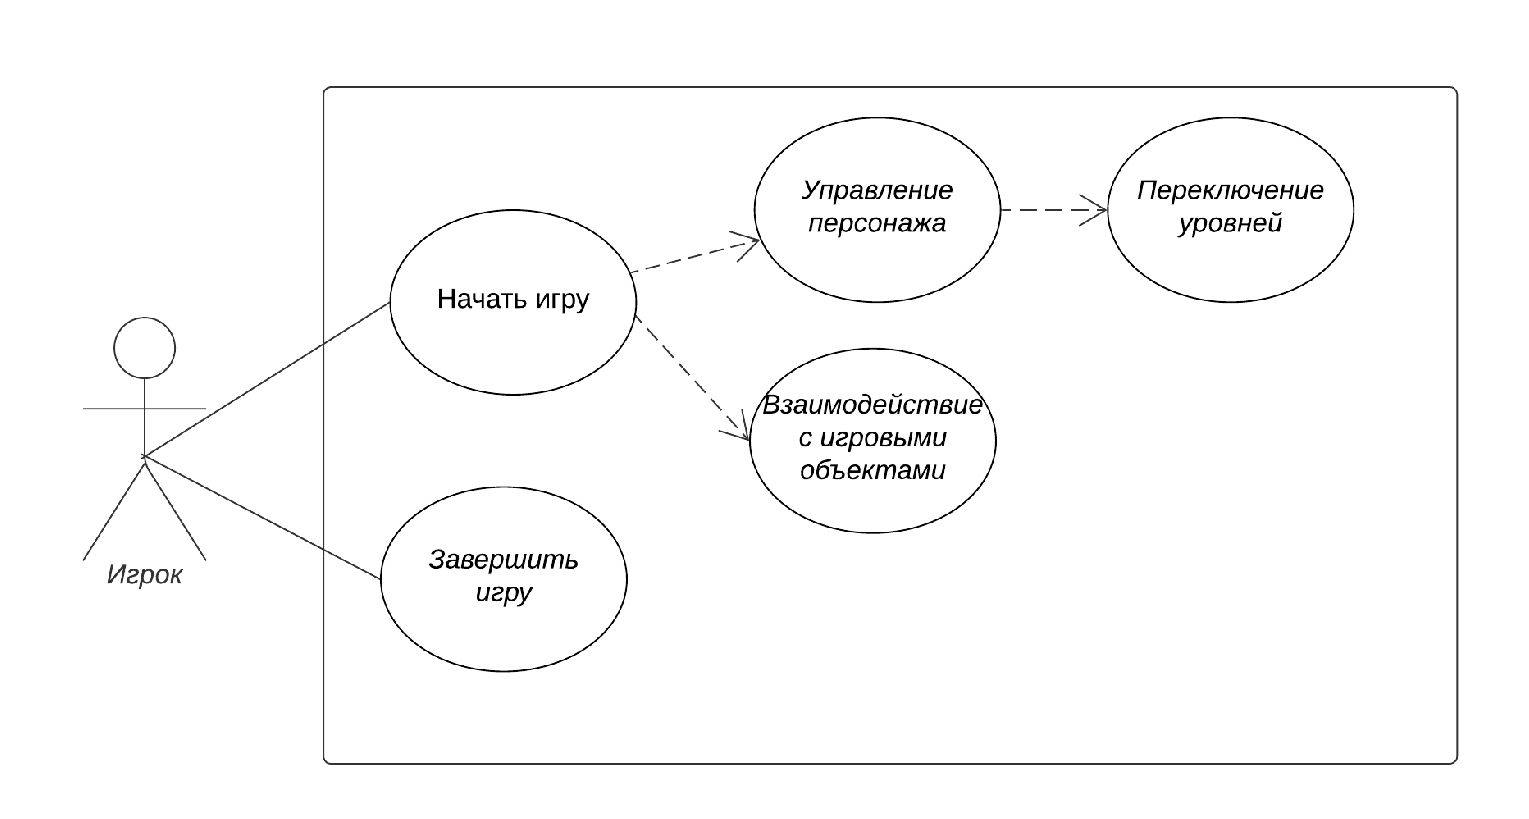
\includegraphics[width=1\linewidth]{precend}}
	\caption{Диаграмма прецедентов}
	\label{precend:image}
\end{figure}

\subsection{Требования к оформлению документации}

Разработка программной документации и программного изделия должна производиться согласно ГОСТ 19.102-77 и ГОСТ 34.601-90. Единая система программной документации.

\section{Технический проект}
\subsection{Технические детали}
Язык программирования: Проект написан на языке программирования Python.

Библиотеки: Проект использует библиотеку SDL2 для графики и обработки событий.

Модули и классы: В коде проекта определены следующие модули и классы:
1. graph-engine:
Функции:создание и настройка графического окна, отрисовка и удаление спрайтов, обработка нажатий на клафиши.
Классы:Graphics: Инициализирует графическое окно, загружает изображения спрайтов, отрисовывает спрайты на экране, обрабатывает события SDL, и завершает работу графической подсистемы SDL.
2. level:
Классы:
Level: Хранит данные об уровне, имеет методы для создания и заполнения уровня тайлами.
LevelAllBricks: Наследуется от Level, определяет конкретный уровень, заполненный одним типом тайлов.
LevelCoridor: Наследуется от LevelAllBricks, определяет уровень с проходом (коридором) из тайлов.
3. the-world:
Классы:
World: Предоставляет функциональность для управления игровыми объектами, добавления/удаления объектов, их обновления и получения информации о них.
4. game-object:
Классы:
GameObject: Определяет базовый игровой объект, его позицию и скорость обновления.
Основной файл main.py:
Импортирует необходимые модули и классы.
Создает экземпляр игры Montezuma и запускает ее.

\subsection{Структура проекта}

\begin{figure}[H]
\centering
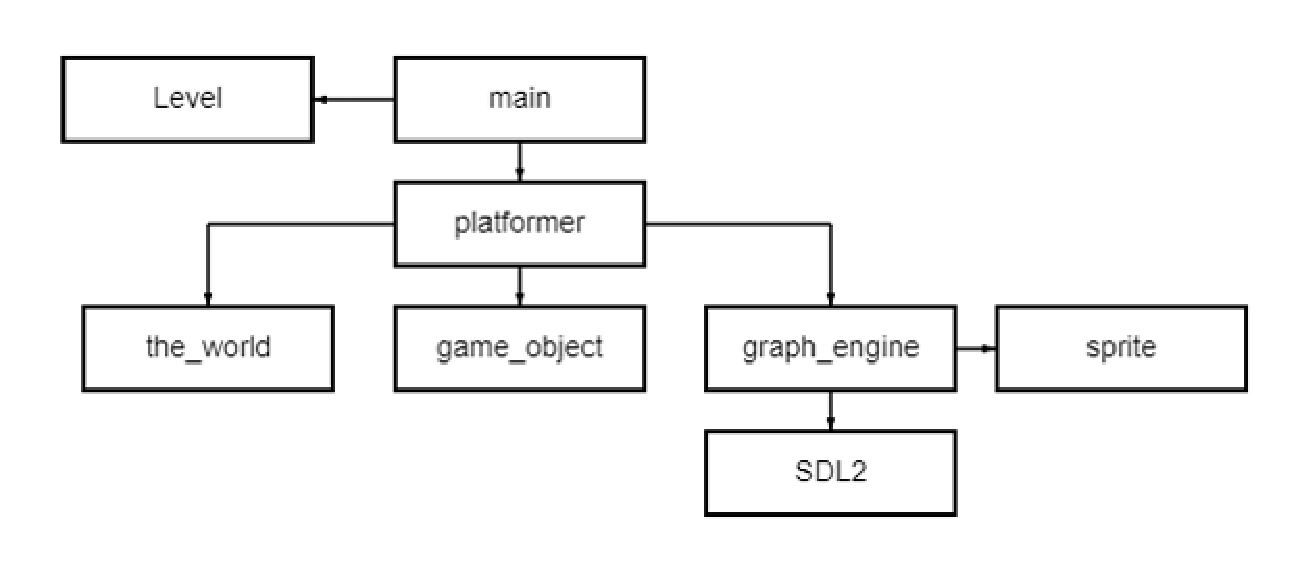
\includegraphics[width=1.05\linewidth]{images/dig1}
\caption{Структура программы}
\label{fig:dig1}
\end{figure}

\begin{figure}[H]
	\center{\includegraphics[width=1.0\linewidth]{UMLMontezuma}}
	\caption{Диаграмма классов}
	\label{UMLMontezuma:image}
\end{figure}

Главный файл main.py: В этом файле вызываются все необходимые модули.

Модуль graph-engine: Модуль для создания и настройки графического окна, создание и отрисовку спрайтоа.

Модуль platformer: Инициализирует графику и запускает игровой цикл.

Модуль the-world: Управляет игровыми объектами, их обновлением и изменением их состояния.

Модуль gameobject: Содержит базовый класс для игровых объектов, определяет их позицию, скорость и обновление.

Модуль sprite: Содержит базовый класс для спрайтов, определяет их позицию и их изображение.

Модуль level: Содержит конфигурацию игровых уровней. 

RESOURCES - объект, предоставляющий доступ к ресурсам (изображениям).

Папка Images: В этой папке содержатся изображения, используемые в игре (например, изображения фона, блоков и персонажа).
\ifПрактика{}\else{
   \section{Рабочий проект}
\subsection{Классы, используемые при разработке сайта}

Можно выделить следующий список классов и их методов, использованных при разработке web-приложения (таблица \ref{class:table}). Пример таблицы с уменьшенным межстрочным интервалом.

\renewcommand{\arraystretch}{0.8} % уменьшение расстояний до сетки таблицы
\begin{xltabular}{\textwidth}{|X|p{2.5cm}|>{\setlength{\baselineskip}{0.7\baselineskip}}p{4.85cm}|>{\setlength{\baselineskip}{0.7\baselineskip}}p{4.85cm}|}
\caption{Описание классов Bitrix, используемых в приложении\label{class:table}}\\
\hline \centrow \setlength{\baselineskip}{0.7\baselineskip} Название класса & \centrow \setlength{\baselineskip}{0.7\baselineskip} Модуль, к которому относится класс & \centrow Описание класса & \centrow Методы \\
\hline \centrow 1 & \centrow 2 & \centrow 3 & \centrow 4\\ \hline
\endfirsthead
\caption*{Продолжение таблицы \ref{class:table}}\\
\hline \centrow 1 & \centrow 2 & \centrow 3 & \centrow 4\\ \hline
\finishhead
CMain & Главный модуль & CMain – главный класс страницы web-приложения. После одного из этапов по загрузке страницы в сценарии становится доступным инициализированный системой объект данного класса с именем \$APPLICATION & void ShowTitle(string property\_code = «title», bool strip\_tags = true)
Выводит заголовок страницы
void SetTitle(string title)
Устанавливает заголовок страницы

void ShowCSS(bool external = true, bool XhtmlStyle = true)
Выводит таблицу стилей CSS страницы\\
\hline CFile & Главный модуль & CFile – Класс для работы с файлами и изображениями & array GetFileArray (int file\_id)
Метод возвращает массив, содержащий описание файла (путь к файлу, имя файла, размер) с идентификатором file\_id
\end{xltabular}
\renewcommand{\arraystretch}{1.0} % восстановление сетки

\subsection{Модульное тестирование разработанного web-сайта}

Модульный тест для класса User из модели данных представлен на рисунке \ref{unitUser:image}.

\begin{figure}[ht]
\begin{lstlisting}[language=Python]
from django.test import TestCase
from .models import *
User = get_user_model()


class ShpoTestCases(TestCase):

    def setUp(self) -> None:
        self.user = User.objects.create(username='testtestovich', password='testtestovich', first_name='Sad', last_name='')

    def test_2(self):

        self.assertEqual(self.user.first_name, 'Sad')
        self.assertEqual(self.user.last_name, 'Cat')
        print((self.user))
        print((self.user.first_name))
        print((self.user.last_name))
\end{lstlisting}  
\caption{Модульный тест класса User}
\label{unitUser:image}
\end{figure}

\subsection{Системное тестирование разработанного web-сайта}

На рисунке \ref{main:image} представлена главная страница сайта «Русатом – Аддитивные технологии».
\newpage % при необходимости можно переносить рисунок на новую страницу
\begin{figure}[H] % H - рисунок обязательно здесь, или переносится, оставляя пустоту
\center{\includegraphics[width=1\linewidth]{main1}}
\center{\includegraphics[width=1\linewidth]{main2}}
\center{\includegraphics[width=1\linewidth]{main3}}
\caption{Главная страница сайта «Русатом – Аддитивные технологии»}
\label{main:image}
\end{figure}

На рисунке \ref{menu:image} представлен динамический вывод заголовков, включающий в себя искомые фразы при поиске фраз.

\begin{figure}[ht]
\center{\includegraphics[width=1\linewidth]{menu}}
\caption{Динамический вывод заголовков}
\label{menu:image}
\end{figure}

На рисунке \ref{enter:image} представлен ввод данных для публикации новости.

\begin{figure}[ht]
\center{\includegraphics[width=1\linewidth]{enter}}
\caption{Ввод данных для публикации очень-очень длинной, интересной и полезной новости}
\label{enter:image}
\end{figure}

   \section*{ЗАКЛЮЧЕНИЕ}
\addcontentsline{toc}{section}{ЗАКЛЮЧЕНИЕ}

Преимущества аддитивных технологий заключается в разнообразии процессов, позволяющих применять их в различных областях производства. Существенным ограничением же является и экономическая составляющая, которая не позволит внедрить аддитивное производство повсеместно.
  
Компании, видя, как развиваются информационные технологии, пытаются использовать их выгодно для своего бизнеса, запуская свой сайт для того, чтобы заявить о своем существовании, проинформировать потенциального клиента об услугах или продуктах, которые предоставляет. 
Для продвижения компании «Русатом – Аддитивные технологии» был разработан веб-сайт на основе системы «1С-Битрикс: Управление сайтом».

Основные результаты работы:

\begin{enumerate}
\item Проведен анализ предметной области. Выявлена необходимость использовать 1С-Битрикс.
\item Разработана концептуальная модель web-сайта. Разработана модель данных системы. Определены требования к системе.
\item Осуществлено проектирование web-сайта. Разработана архитектура серверной части. Разработан пользовательский интерфейс web-сайта.
\item Реализован и протестирован web-сайт. Проведено модульное и системное тестирование.
\end{enumerate}

Все требования, объявленные в техническом задании, были полностью реализованы, все задачи, поставленные в начале разработки проекта, были также решены.

Готовый рабочий проект представлен адаптивной версткой сайта. Сайт находится в публичном доступе, поскольку опубликован в сети Интернет.  

}\fi
\addcontentsline{toc}{section}{СПИСОК ИСПОЛЬЗОВАННЫХ ИСТОЧНИКОВ}

\begin{thebibliography}{9}

    \bibitem{javascript} Фримен, А. Практикум по программированию на JavaScript / А. Фримен. – Москва~: Вильямс, 2013. – 960 с. – ISBN 978-5-8459-1799-7. – Текст~: непосредственный.
    \bibitem{php} Бретт, М. PHP и MySQL. Исчерпывающее руководство / М. Бретт. – Санкт-Петербург : Питер, 2016. – 544 с. – ISBN 978-5-496-01049-8. – Текст~: непосредственный.
    \bibitem{css} Веру, Л. Секреты CSS. Идеальные решения ежедневных задач / Л. Веру. – Санкт-Петербург : Питер, 2016. – 336 с. – ISBN 978-5-496-02082-4. – Текст~: непосредственный.
    \bibitem{mysql}	Гизберт, Д. PHP и MySQL / Д. Гизберт. – Москва~: НТ Пресс, 2013. – 320 с. – ISBN 978-5-477-01174-2. – Текст~: непосредственный.
	\bibitem{html5}	Голдстайн, А. HTML5 и CSS3 для всех / А. Голдстайн, Л. Лазарис, Э. Уэйл. – Москва~: Вильямс, 2012. – 368 с. – ISBN 978-5-699-57580-0. – Текст~: непосредственный.
	\bibitem{htmlcss}	Дэкетт, Д. HTML и CSS. Разработка и создание веб-сайтов / Д. Дэкетт. – Москва~: Эксмо, 2014. – 480 с. – ISBN 978-5-699-64193-2. – Текст~: непосредственный.
	\bibitem{bigbook}	Макфарланд, Д. Большая книга CSS / Д. Макфарланд. – Санкт-Петербург : Питер, 2012. – 560 с. – ISBN 978-5-496-02080-0. – Текст~: непосредственный.
	\bibitem{uchiru}	Лоусон, Б. Изучаем HTML5. Библиотека специалиста / Б. Лоусон, Р. Шарп. – Санкт-Петербург : Питер, 2013 – 286 с. – ISBN 978-5-459-01156-2. – Текст~: непосредственный.
	\bibitem{chaynik}	Титтел, Э. HTML5 и CSS3 для чайников / Э. Титтел, К. Минник. – Москва~: Вильямс, 2016 – 400 с. – ISBN 978-1-118-65720-1. – Текст~: непосредственный.    
	\bibitem{22}	Титтел, Э. HTML5 и CSS3 для чайников / Э. Титтел, К. Минник. – Москва~: Вильямс, 2016 – 400 с. – ISBN 978-1-118-65720-1. – Текст~: непосредственный.    
	\bibitem{1231}	Титтел, Э. HTML5 и CSS3 для чайников / Э. Титтел, К. Минник. – Москва~: Вильямс, 2016 – 400 с. – ISBN 978-1-118-65720-1. – Текст~: непосредственный.    
	\bibitem{sdf}	Титтел, Э. HTML5 и CSS3 для чайников / Э. Титтел, К. Минник. – Москва~: Вильямс, 2016 – 400 с. – ISBN 978-1-118-65720-1. – Текст~: непосредственный.    
	\bibitem{servsssds}	Титтел, Э. HTML5 и CSS3 для чайников / Э. Титтел, К. Минник. – Москва~: Вильямс, 2016 – 400 с. – ISBN 978-1-118-65720-1. – Текст~: непосредственный.
\end{thebibliography}

\ifВКР{\appendix{Представление графического материала}

Графический материал, выполненный на отдельных листах,
изображен на рисунках А.1--А.\arabic{числоПлакатов}.
\setcounter{числоПлакатов}{0}

\renewcommand{\thefigure}{А.\arabic{figure}} % шаблон номера для плакатов

\begin{landscape}

\begin{плакат}
    
\includegraphics[width=0.82\linewidth]{плакат1.png}
    \заголовок{Сведения о ВКРБ}
    \label{pl1:image}      
\end{плакат}

\begin{плакат}
    
\includegraphics[width=0.82\linewidth]{плакат2.png}
    \заголовок{Цель и задачи разработки}
    \label{pl2:image}      
\end{плакат}

\begin{плакат}
    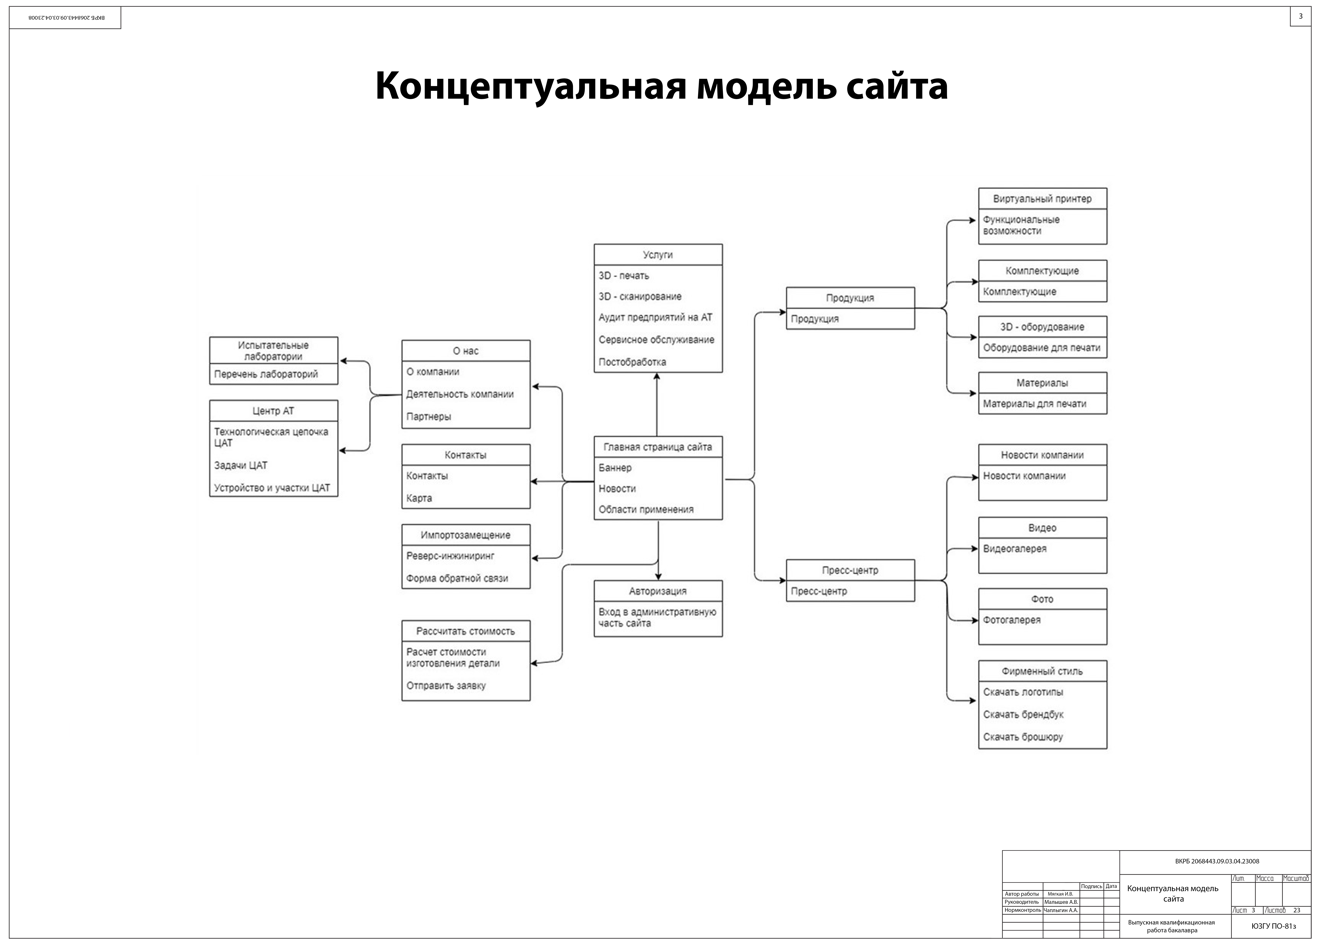
\includegraphics[width=0.82\linewidth]{плакат3.png}
    \заголовок{Концептуальная модель сайта}
    \label{pl3:image}      
\end{плакат}

\begin{плакат}
    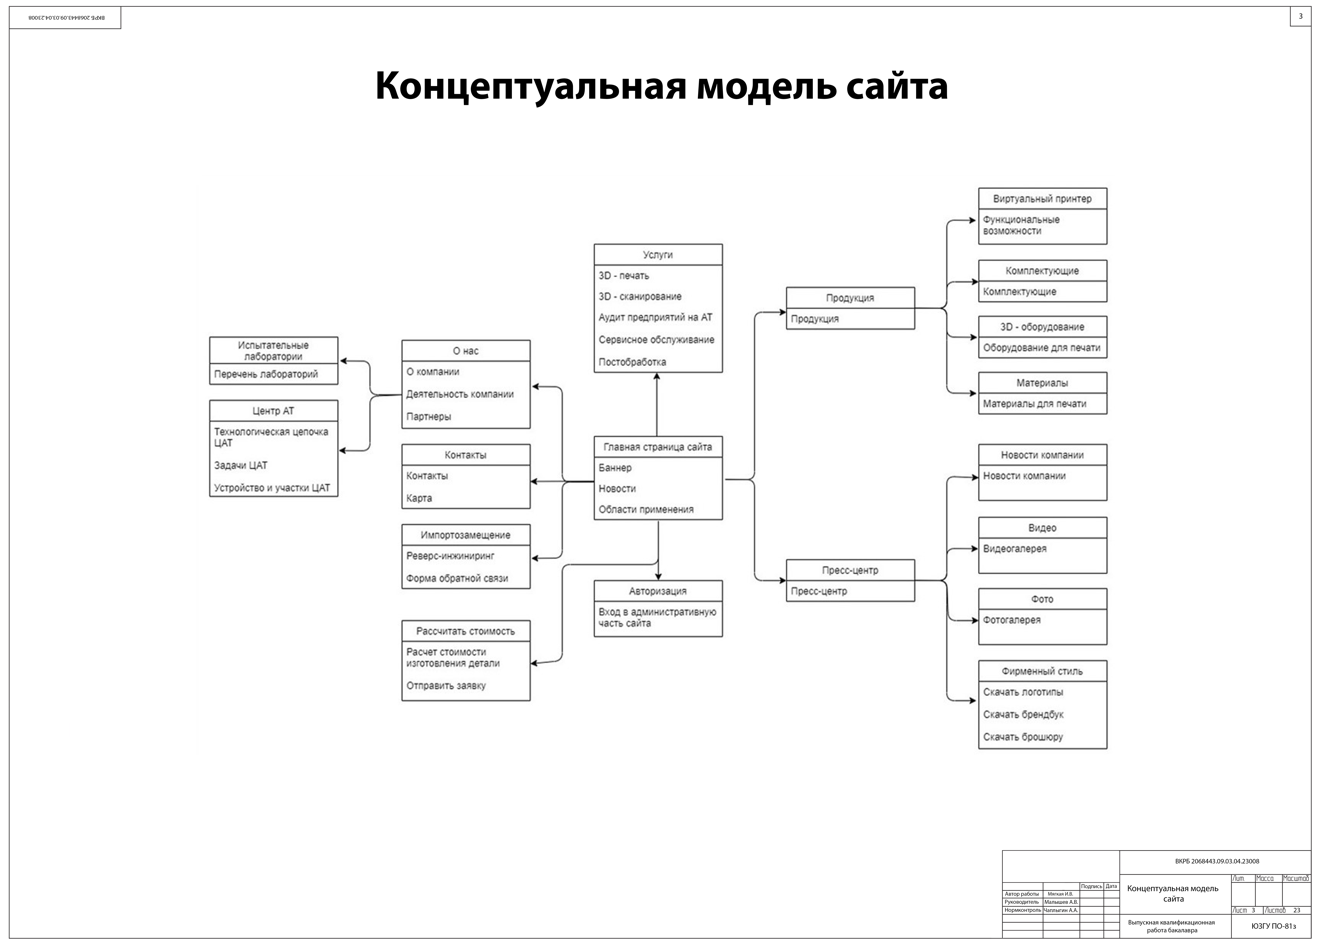
\includegraphics[width=0.82\linewidth]{плакат3.png}
    \заголовок{Еще плакат}
    \label{pl4:image}      
\end{плакат}

\end{landscape}
}\fi
\ifПрактика{}\else{\appendix{Фрагменты исходного кода программы}

main.tex
\lstinputlisting[language=Tex, frame=none]{main.tex}

ТехПроект.tex
\lstinputlisting[language=Tex, frame=none]{ТехПроект.tex}

\ifВКР{
\newpage
\addcontentsline{toc}{section}{На отдельных листах (CD-RW в прикрепленном конверте)}
\begin{center}
\textbf{Место для диска}
\end{center}
}\fi
}\fi
\end{document}
